\section{Conceptual Design and Development}
\label{sec:conceptualDesign}
  It was clear from the list of specifications that both electrical and mechanical aspects of the project required development of a large number of parts. In a typical conceptual design process, one could propose a number of complete concepts (i.e. incorporating all aspects of the project) and then make a judgement based on analysis of these concepts. For this project, it was decided that each of the subcomponents outlined in the specifications be conceptually envisioned separately with consideration of neighbouring or related subcomponents and the compatibility between each. Analysis was then undertaken for each of the subcomponents and a final design was composed in a convergent manner, taking the best concept from each of the analyses.
  
  The project requirement to produce a high-fidelity replica of \textit{Curiosity} helped to maintain structure during a highly parallel, componentised conceptual development. However, the majority of the software components and some hardware components relied on the design of other components therefore the design process was not \textit{entirely} parallel. In fact, in the case of the vehicle development, it was due to it being largely a process of replication that most of the conceptual development involved material and manufacture design choices, as opposed to new conceptual ideas that would have required analysis of design feasibility.
  
  After descriptions of each of the component concepts, a weighted comparative analysis was performed and the results of each of these analyses is tabulated. A selection of attributes relevant to each component was given a weight on a scale of one to five indicating the importance of the attribute to the design. Each of the concepts was given a score for each attribute. A weighted sum of each of the concepts' scores resulted in a final score used to determine which concept was more suitable for the design.
  
  \subsection{Rover Concept Proposals}
  \label{subsec:rover-concept-proposals}    
    \subsubsection{Body}
      All of the proposed ideas for the body component of the model revolved around the idea of a hollow box structure. The box was required to host electronics but at the same time, provide structural stability for all other components that were to be mounted to it. Therefore, the choice here was between the materials from which it would be built.
      
      \subheading{Concepts}
      \begin{enumerate}
        \item \textbf{Carbon Fibre:} The first idea envisioned the use of carbon fibre to form a box structure that could be very thin and light but still offer the required strength. The carbon fibre would be cured around a mould made from another rigid, easy to use material. When rigid, holes would be drilled for mounting components and electronics. This concept includes the use of fibre glass which is commonly interchanged with carbon fibre. Both materials offer similar tensile strength, however, carbon fibre is far more robust in flexure \cite{fibreGlast_2016}.
        
        \item \textbf{Perspex/Acrylic Sheet Assembly:} The next idea involved creating the box by designing and cutting panels from acrylic sheet of acceptable thickness, and later fusing the panels to form the structure. Cut-outs could have been included in the design together with holes for shafts and mounting points, which may also have been drilled after the fact. Internal support structures could have been included if the strength of the bonds or of the structure in general was in question due to the fact that acrylic sheet offers high flexibility.
        
        \item \textbf{3D Printing:} One of the aims of the project was to develop the model with high realism in an attempt to make the use of the simulator an engaging and appealing experience. The idea of 3D printing the box structure was considered and it would have allowed for a large degree of detail to be included at little additional effort or cost. Most features such as mounting points (those beyond just holes) and aesthetic detail could have been designed on top of base and internal structural support. A material could have been chosen which might offer the required rigidity, however, due to the nature of the manufacturing process, specifically the reliance on heat for the deforming of the plastic filament in the printing process, 3D printed components would not provide the same strength and robustness as compared to that of the other concepts. A 3D model intended for 3D printing of \textit{Curiosity} created and published by NASA was found \cite{nasa3Dprint}. Of specific interest was the body component which shows the detail that is achievable with this method, a render of which is in Figure~\ref{fig:concepts-nasa3DReferenceBody}.
        
        \begin{figure}[h!]
          \centering
          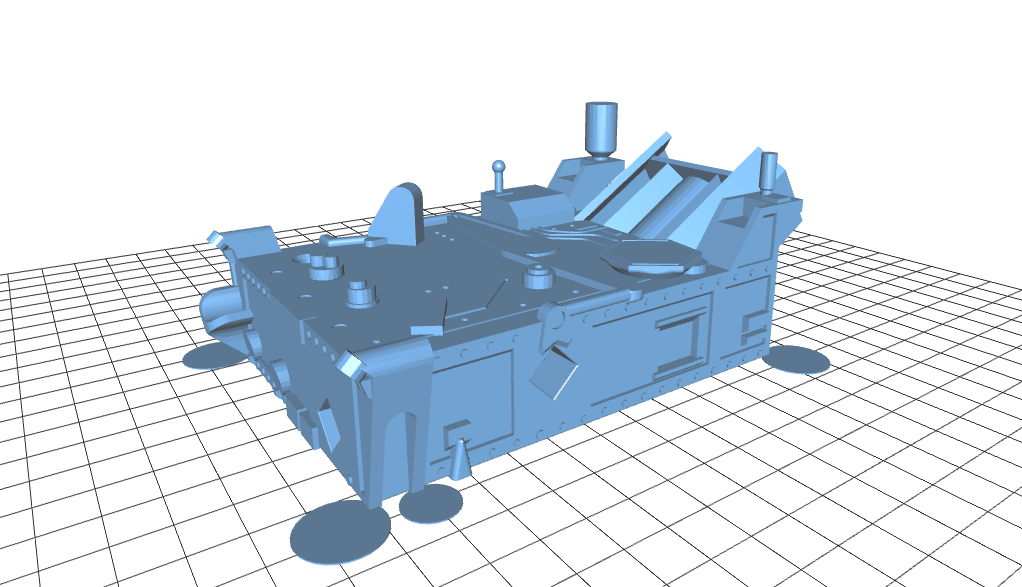
\includegraphics[width=0.8\linewidth]{figures/concepts-nasa3DReferenceBody}
          \caption[3D render of the body component of the model provided by NASA intended for additive replication.]{3D render of the body component of the model provided by NASA intended for additive replication \cite{nasa3Dprint}.}
          \label{fig:concepts-nasa3DReferenceBody}
        \end{figure}
        
        \item \textbf{Milled Aluminium:} Aluminium was another concept that was considered due to its improved manipulative properties (compared to those of steel) as well as significant reductions in weight. The box structure could have been milled from a block to form the hollow structure that is required, using CNC technology. Holes for mounting and a fair degree of aesthetic detail, which may not have lived up to that achievable by 3D printing means, may have been possible as well. Having the box structure made from aluminium would have meant that threaded holes for mounting would have been possible, eliminating the need for full-stack fasteners.
      \end{enumerate}
      
      \subheading{Discussion}\\\\
      All of the above concepts were practical, however, each drew on very different material requirements and manufacturing techniques. Carbon fibre moulding and setting was seen as being a potentially difficult process in terms of ensuring an accurate outcome as it relied on a larger degree of manual manufacturing input. It was also the only idea that required extra components to be manufactured in support, namely the mould around which it would have been formed. The other three concepts allowed for more direct CAD-to-finished-product processes and the automation involved in the manufacture of them meant higher accuracy and less manual input. Since the model was small in scale (a design choice discussed further on in this report) strength of components and the weight of other components was far less of a priority as compared to resistance to heat and level of detail.
      
      \subheading{Comparative Analysis}\\\\
      A comparative analysis of the four options for the design and manufacture of the body is shown in Table~\ref{tab:concept-compAnalysisBody}.
      
      \begin{table}[H]
      \centering
      \begin{tabular}{@{}L{0.3\textwidth}C{0.12\textwidth}C{0.12\textwidth}C{0.12\textwidth}C{0.12\textwidth}C{0.12\textwidth}@{}}
      \toprule
      Attribute & Weight & Carbon Fibre & Acrylic Sheet Assembly & 3D Printing & Milled Aluminium \\ \midrule
      Ease of Manufacture & 5 & 1 & 5 & 3 & 4 \\
      Cost of Manufacture & 4 & 4 & 5 & 3 & 4 \\
      Duration of Manufacture & 5 & 4 & 5 & 3 & 4 \\
      Cost of Material & 4 & 2 & 4 & 3 & 3 \\
      Weight & 5 & 5 & 5 & 4 & 2 \\
      Tensile Strength & 2 & 4 & 3 & 3 & 5 \\
      Modulus & 3 & 5 & 4 & 4 & 1 \\
      Achievable Detail & 3 & 1 & 1 & 5 & 4 \\
      Achievable Accuracy & 3 & 1 & 3 & 4 & 5 \\ \midrule
      \multicolumn{2}{r}{\textbf{Total}} & 2.735 & \textbf{4.147} & 3.353 & 3.324 \\ \bottomrule
      \end{tabular}
      \caption{Comparative analysis of the body component concepts.}
      \label{tab:concept-compAnalysisBody}
      \end{table}
    \subsubsection{Suspension System}
      The suspension system of the rover was a critical part with respect to the traversal requirements. It was decided up front that the rover should replicate this feature as it was on \textit{Curiosity} in both appearance and in operation. The Rocker-bogie mechanical principle employed for the \textit{Curiosity's} suspension system was simple and robust and therefore made clear the decision to use the principle in the model as well. The design problem here was more concerned with the structure and material of the joints as well as how they would be fitted with the beams/rods that links the system together. Another design consideration was that of the differential cross-beam mounted to the top of \textit{Curiosity} which articulates around a center point. The choice of differential bar was dealt with in a separate analysis.
      
      All of the concepts discussed below imply the use of shafts and bearings for free articulation between each of the rocker-bogie sections.
      
      \subheading{Concepts}
      \begin{itemize}
        \item \textbf{Fully 3D Printed Assembly:} In this concept, all the parts were to be 3D printed in full. This meant that the joints and beams of the suspension system were not separate pieces, lowering the number of pieces required to be manufactured. Since the suspension system was the largest load bearer compared to that of the other subsystems, the fully printed pieces could have been reinforced with an aluminium or steel rod set down the center of the beam sections. The reinforcements could have extended partially into the joint section of each piece, as the most amount of structural risk would have been at the point where the joint and the beam meet.
        
        \item \textbf{Printed Joints with Aluminium Tubing:} Instead of printing the entire system, an option of printing the joints only and fitting them with aluminium tubing, as the beams, was considered. 3D printing provides the benefit of being able to materialise complex objects which may contain features which conventional manufacture methods might not be able to accomplish, thus making it well suited to the unique nature of the joints in the suspension system. The beams, however, were standard in shape and would not have put this benefit to use, hence motivating the suitability of a light but strong product such as aluminium tubing. The joints would have been designed either to have the tubing fit into the joint, or have a plug onto which the tubing could be pressed.
      
        \item \textbf{Sheet Brackets with Aluminium Tubing:} This concept built on the previous concept with the joints being made from sheet metal bent into bracket-type shapes onto which the tubing could have been fastened (by means of clamps). The bending process would have allowed for formation of the non-conventional angles that the suspension system required.
        
        \item \textbf{Milled Aluminium Joints with Aluminium Tubing:} Again, instead of the 3D printed joints or the sheet metal, this concept made use of milling aluminium to form the joint structures and having aluminium tubing be fitted into these joints. The milled joints would have been able to offer more surface area to features such as mounting points for the tubes and bearings, meaning that these parts would be more secure. This idea, shown in Figure~\ref{fig:concepts-openCuriosityMachinedJoints}, was borrowed from the OpenCuriosity project \cite{opencuriosity2014} as highlighted in Section~\ref{chap:lit-review}.
        
        \begin{figure}[h!]
          \centering
          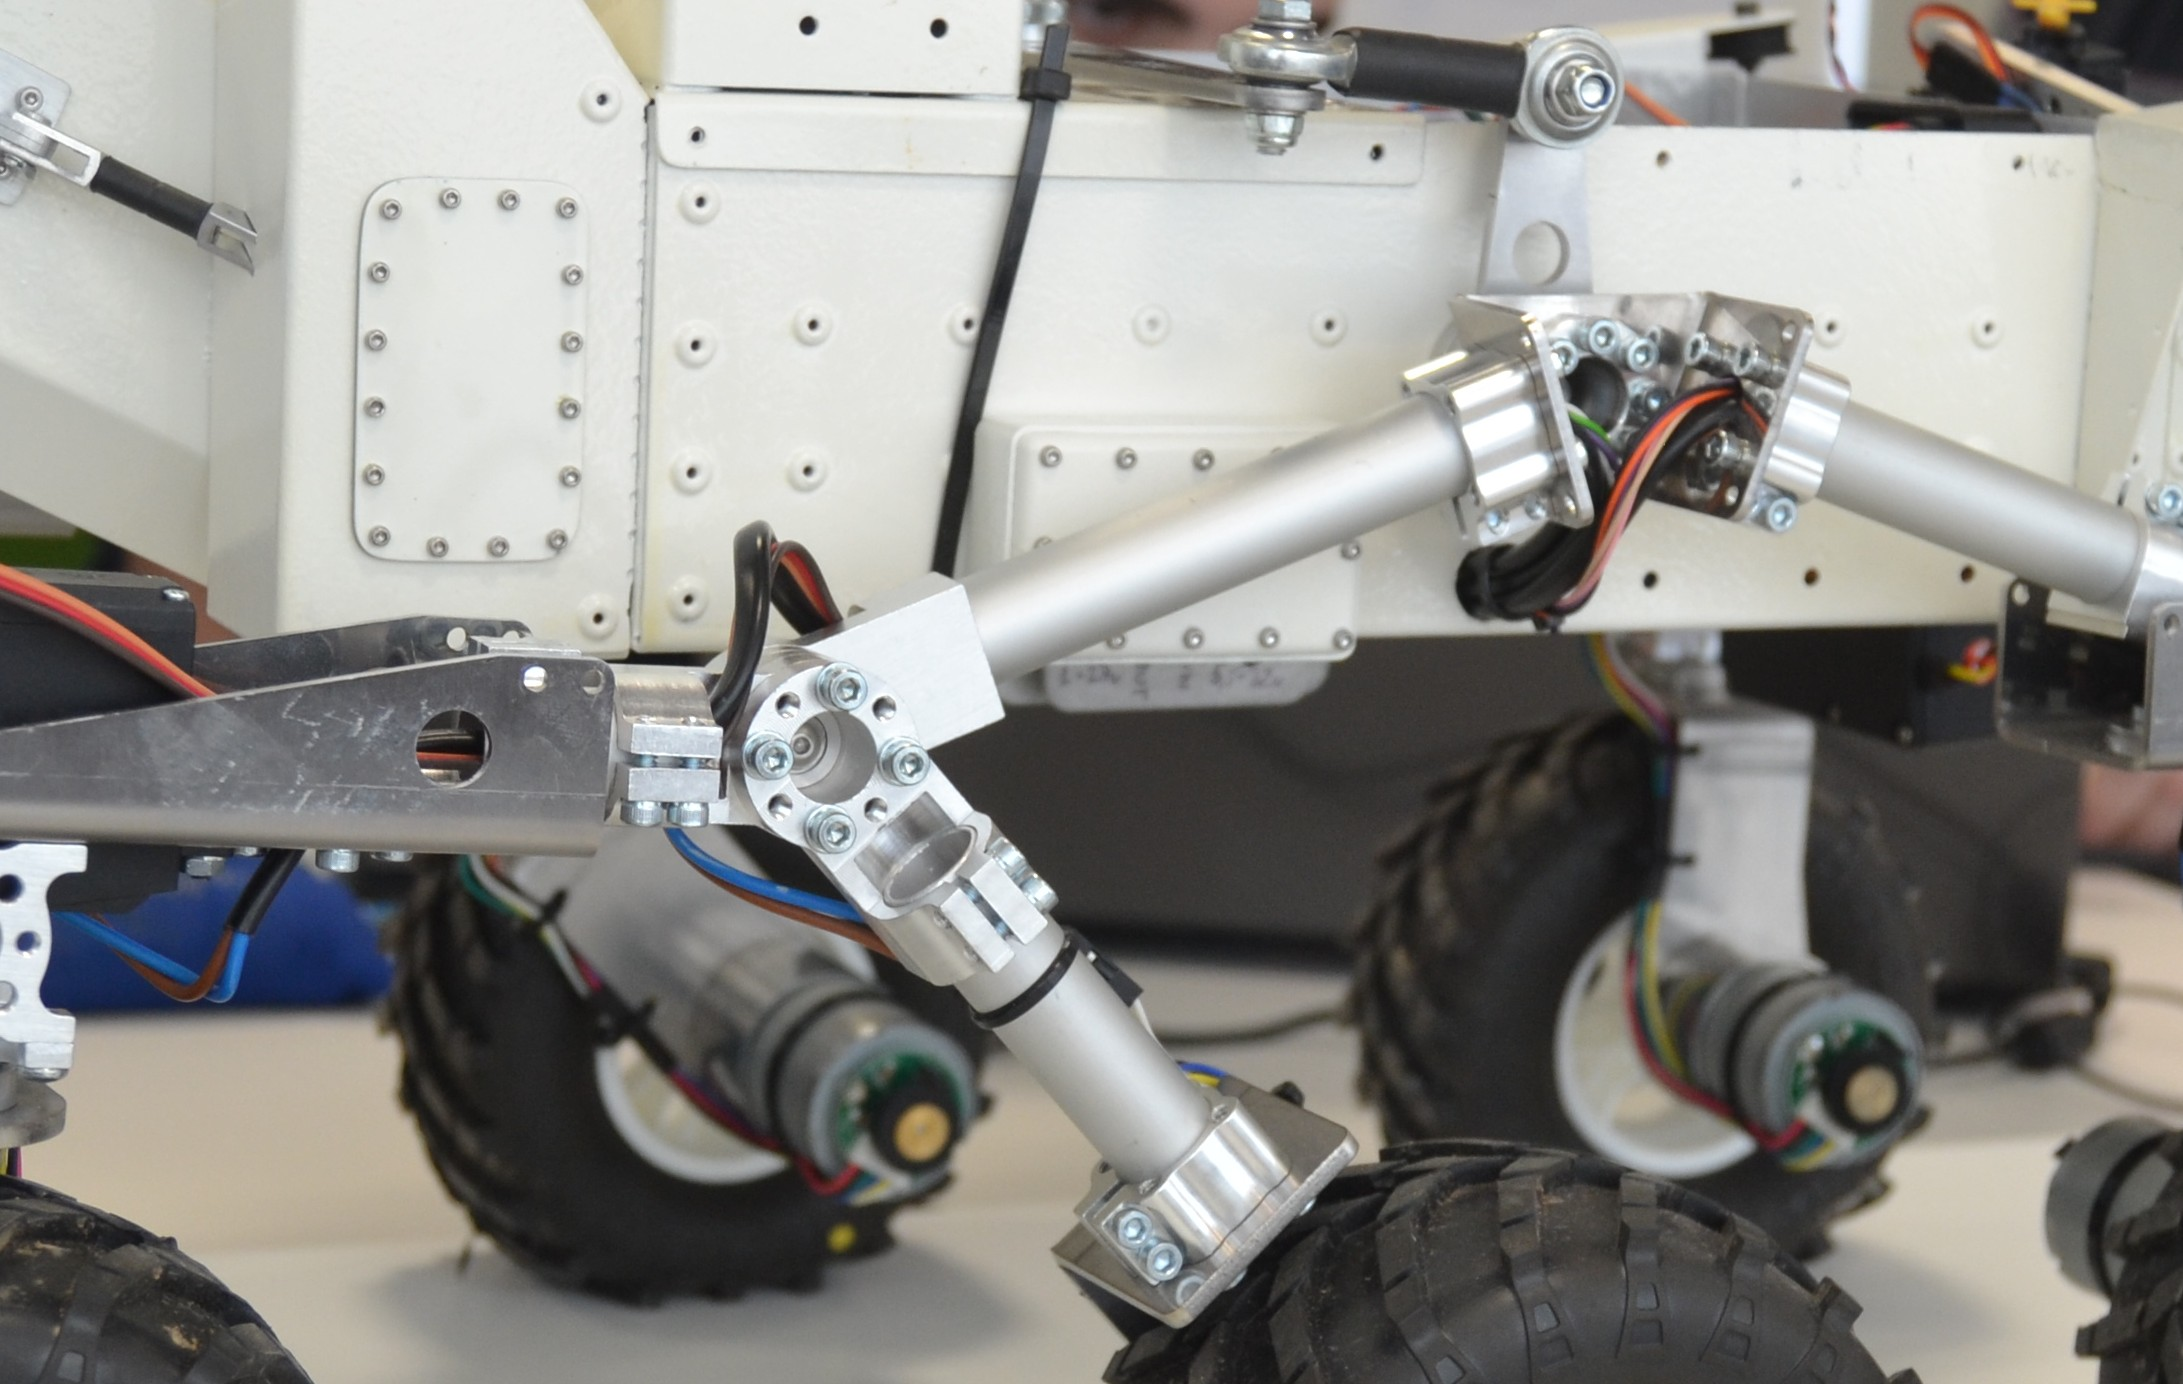
\includegraphics[width=0.7\linewidth]{figures/concepts-openCuriosityMachinedJoints}
          \caption[Image showing the machined joints used on the OpenCuriosity rover model.]{Image showing the machined joints used on the OpenCuriosity rover model \cite{opencuriosity2014}.}
          \label{fig:concepts-openCuriosityMachinedJoints}
        \end{figure}
        
      \end{itemize}

      \subheading{Discussion}\\\\
      The fully 3D printed concept was appealing in that it offered the most direct path from CAD design to the finished product but had much reduced structural qualities as opposed to that of the other concepts. Using a combination of tubing and manufactured joints made sense in terms of the nature of the features and aluminium tubing provided strength beyond what was required, at least as far as the tubing itself was concerned. Brackets made from sheet metal may have offered the best weight (that is, the lightest weight contribution) but required extra manual manufacture and would not have been suited to mounting bearings and the tubes whilst maintaining mount rigidity. Both milled aluminium and 3D printed joints solved this problem with the ability of being able to provide more rigidity for fastening tubes and fitting bearings. However, milled joints were bound in structure to the block of aluminium from which they were to be milled, meaning that in one particular plane, the axes of the joints would not have been able to be angled such as required by the suspension design.
      
      \subheading{Comparative Analysis}\\\\
      A comparative analysis of these four options of design and manufacture of the suspension system is shown in Table~\ref{tab:concept-compAnalysisSus}.
      
      \begin{table}[H]
      \centering
      \begin{tabular}{@{}L{0.3\textwidth}C{0.12\textwidth}C{0.12\textwidth}C{0.12\textwidth}C{0.12\textwidth}C{0.12\textwidth}@{}}
      \toprule
      Attribute & Weight & Full 3D Print & 3D Printed Joints w/ Tubing & Sheet Joints w/ Tubing & Milled Joints w/ Tubing \\ \midrule
      Ease of Manufacture & 5 & 4 & 3 & 2 & 3 \\
      Duration of Manufacture & 3 & 2 & 4 & 5 & 3 \\
      Cost of Manufacture & 4 & 2 & 3 & 4 & 3 \\
      Cost of Material & 4 & 3 & 4 & 5 & 4 \\
      Weight & 4 & 4 & 4 & 3 & 2 \\
      Link Mount Rigidity & 5 & 3 & 4 & 1 & 5 \\
      Aesthetic Accuracy & 3 & 5 & 5 & 1 & 3 \\
      Suitability for Wheel Mounts & 4 & 5 & 5 & 4 & 5 \\ \midrule
      \multicolumn{2}{r}{\textbf{Total}} & 3.500 & \textbf{3.938} & 3.031 & 3.563 \\ \bottomrule      
      \end{tabular}
      \caption{Comparative analysis of the suspension system concepts.}
      \label{tab:concept-compAnalysisSus}
      \end{table}
      
    \subsubsection{Differential System}
      The differential system on \textit{Curiosity} comprises a beam or arm that articulates about a centre point on the top surface of the body and linkage mechanisms connecting the ends of the arm to the rocker pivot point on either side's suspension system. Due to the motion of the differential, strength is only required in the horizontal plane which gives reason for the thin, flat design of \textit{Curiosity}. Once again, the principle of operation of this subsystem was taken from \textit{Curiosity} itself and therefore was not the design choice to be made here. Considered were several possible material options to implement the differential bar on the rover. The linkages on the ends of the bar required hinges with two degrees of freedom, the detail of which is discussed further on in this report.
      
      \subheading{Concepts}
      \begin{itemize}
        \item \textbf{Acrylic Sheet Bar with Steel Cord Linkage:} Since the differential bar was required to take forces in the horizontal plane, the bar did not have to be round and a conceptual idea involved cutting out the flat bar from acrylic sheet. The acrylic sheet would have been thick enough to be press fitted onto a bearing and shaft in the centre of the body deck. The ends of the differential bar would then have been connected to the extensions on the main suspension joint by means of steel cord. The cord would have allowed for the degrees of freedom required given the interface between the differential bar and the suspension and each of their component axes of motion.
        
        \item \textbf{3D Printed Bar with 3D Printed Hinge Pieces:} Instead of cutting the bar from acrylic sheet, this concept envisioned the bar being 3D printed. The linkages would have also been 3D printed as two parts per hinge bolted together and each end of the hinge (one at the suspension and one on the differential bar) would be joined together using threaded bar, secured by use of fasteners.
      \end{itemize}
      
      \subheading{Discussion}\\\\
      Since the acrylic sheet is already flat, it suits the requirement well and is easier in terms of manufacture compared to a 3D printed version. Holes for the bearings and the hinges on the ends of the bar could be included in the cutting process. Two sheets could have been glued together to form a thicker beam in the case that the bearing was thicker than the sheet. The 3D printed version, however, would have been of designed thickness thus allowing custom fitting for the bearing. Although steel cord was considered given its flexibility and thus ability to cater for the ranges and axes of motion of either ends of the linkage, it was rapidly dismissed given that it would have only been able to provide support in tension and not in compression. A fixed threaded bar, as proposed in the second concept, provides support in both tension and compression situations, therefore meeting the requirements. Threaded bar was chosen for easy fastening as well as providing the ability to adjust the extension of the linkage for fine tuning the balance of the suspension-differential system and ultimately the balance of the rover. In any case, a weighted comparison was still made in Table~\ref{tab:concept-compAnalysisDiff} since the 3D printed hinges were still compatible with the idea an acrylic sheet differential.
      
      \subheading{Comparative Analysis}\\\\
      A comparative analysis of these two options for the design and manufacture of the differential system is shown in Table~\ref{tab:concept-compAnalysisDiff}.
      
      \begin{table}[H]
      \centering
      \begin{tabular}{@{}L{0.3\textwidth}C{0.12\textwidth}C{0.2\textwidth}C{0.2\textwidth}@{}}
      \toprule
      Attribute & Weight & Acrylic Sheet Bar w/ Steel Cord Linkage & 3D Printed Bar w/ Printed Hinge Pieces \\ \midrule
      Ease of Manufacture & 5 & 5 & 3 \\
      Duration of Manufacture & 3 & 5 & 2 \\
      Cost of Manufacture & 4 & 4 & 3 \\
      Cost of Material & 4 & 5 & 3 \\
      Weight & 3 & 5 & 4 \\
      Strength & 5 & 3 & 5 \\
      Mountability & 5 & 3 & 5 \\
      Linkage Motion & 4 & 0 & 4 \\
      Linkage Support & 5 & 5 & 5 \\
      Aesthetic Accuracy & 2 & 1 & 4 \\ \midrule
      \multicolumn{2}{r}{\textbf{Total}} & 3.575 & \textbf{3.900} \\ \bottomrule      \end{tabular}
      \caption{Comparative analysis of the differential concepts.}
      \label{tab:concept-compAnalysisDiff}
      \end{table}
      
    \subsubsection{Wheel Hubs and Pivots}
      The center wheels were fixed in rotation about the $z$-axis and thus the mounting features of these two wheels were included in the suspension system as in the previous concept section. The front and rear wheel pairs, however, were required to rotate in order to provide steering to the rover and therefore had to accommodate for this rotation as well as actuation components for this motion. The wheel pivots were also required to be attached to the suspension system.
      
      The concepts developed for these components followed very similar concepts to those of the suspension hinges as they offered the same principles of articulation and mounting. The final decision would therefore be in accordance with the final design of the suspension system.
      
    \subsubsection{Wheels}
      The wheels on \textit{Curiosity} are signature features in aesthetics as well as, of course, in function. The wheel shape includes the characteristic curved cross-section which has benefits for terrain like that on Mars and are unique in the thinness of their outer surface or skin. It was noted that the relative strength of the wheels on the scaled model that was being developed would be required to be significantly less than on \textit{Curiosity} and so the design choice here was based primarily on the resulting aesthetic accuracy as the wheels would serve as a key feature in which to fulfil the client requirement of the model being highly realistic.
      
      \subheading{Concepts}
      \begin{itemize}
        \item \textbf{3D Printed Wheels:} The fact that the wheels had the distinct shape that they did meant that 3D printing them would render highly accurate representations in terms of their shape compared to those of \textit{Curiosity}. The design would include holes and points at which shafts and/or bearings could be fitted without the need for drilling or any other type of post-produce manipulations.
        
        \item \textbf{Off-the-shelf RC Wheels:} Another option was to purchase ready made wheels and tyres intended for use on radio-controlled cars. The wheels would have points for mounting by default and would offer the benefits of a rubber tyre over that of plastic. Once again, this idea was borrowed from the OpenCuriosity model in \cite{opencuriosity2014}. The project indicated that this method was successful in function.
      \end{itemize}
      
      \subheading{Discussion}\\\\
         While the 3D printed wheels would have offered less structural robustness as ready-made wheels designed to endure high impact, gravel environments, there was no requirement for the model to traverse any faster or in any better manner than \textit{Curiosity} and thus the added benefit of the rubber tyres and strong wheels would be an over-design. Although the RC wheels would have had points at which shafts could be fitted, and potentially even bearings already installed, this would impose limitations on the size of the shafts chosen. In the case of the 3D printed wheels, holes sizes could have been chosen to work with materials and bearings that were available.
         
      \subheading{Comparative Analysis}\\\\
        A comparative analysis of these two options for representing the wheels is shown in Table~\ref{tab:concept-compAnalysisWheel}.
      
        \begin{table}[H]
        \centering
        \begin{tabular}{@{}L{0.3\textwidth}C{0.12\textwidth}C{0.2\textwidth}C{0.2\textwidth}@{}}
        \toprule
        Attribute & Weight & 3D Printed Wheels & Off-the-shelf RC Wheels \\ \midrule
        Ease of Manufacture & 3 & 3 & 5 \\
        Duration of Manufacture & 4 & 2 & 5 \\
        Cost of Manufacture & 4 & 3 & 2 \\
        Cost of Material & 4 & 3 & 2 \\
        Weight & 1 & 5 & 2 \\
        Traction & 3 & 3 & 5 \\
        Terrain Suitability & 3 & 4 & 5 \\
        Mount-type Flexibility & 4 & 5 & 2 \\
        Aesthetic Accuracy & 5 & 5 & 1 \\ \midrule
        \multicolumn{2}{r}{\textbf{Total}}  & \textbf{3.613} & 3.097 \\ \bottomrule
        \end{tabular}
        \caption{Comparative analysis of the wheel and tyre concepts.}
        \label{tab:concept-compAnalysisWheel}
        \end{table}
      
    \subsubsection{Neck and Head}
      The mast of the model required rotation about the $z$-axis and a joint about which an additional axis of rotation was possible to result in two degrees of freedom for the head component. \textit{Curiosity} employed a hinge mounted to the bottom of a second, smaller box structure, the head, which rotated to provide camera pitch. The pitch actuation mechanism was situated atop a second mechanism which provided actuation for pan-axis rotation. The size of \textit{Curiosity} allowed smart fitting of the motors in-line with the mast shaft and embedded in the head mount hinge, however, the scaled model was not able to accommodate motors in this way.
      
      \subheading{Concepts}
      \begin{itemize}
        \item \textbf{Aluminium Tube Mast with 3D Printed Fittings:} This concept made use of aluminium tubing (the same material as in the suspension system concepts) which would be set and fastened into the body. A 3D printed plug with mounting points for the camera-pitch actuation mechanism would have been designed to fit into the top of the tube, as can be seen in Figure~\ref{fig:concepts-aluMast}. Camera-pan actuation would have been built into the inside of the body into which the mast tube would extend. The height of the head could therefore have been adjusted since the tube was free-moving with respect to the rover deck.
        
        \begin{figure}[H]
          \centering
          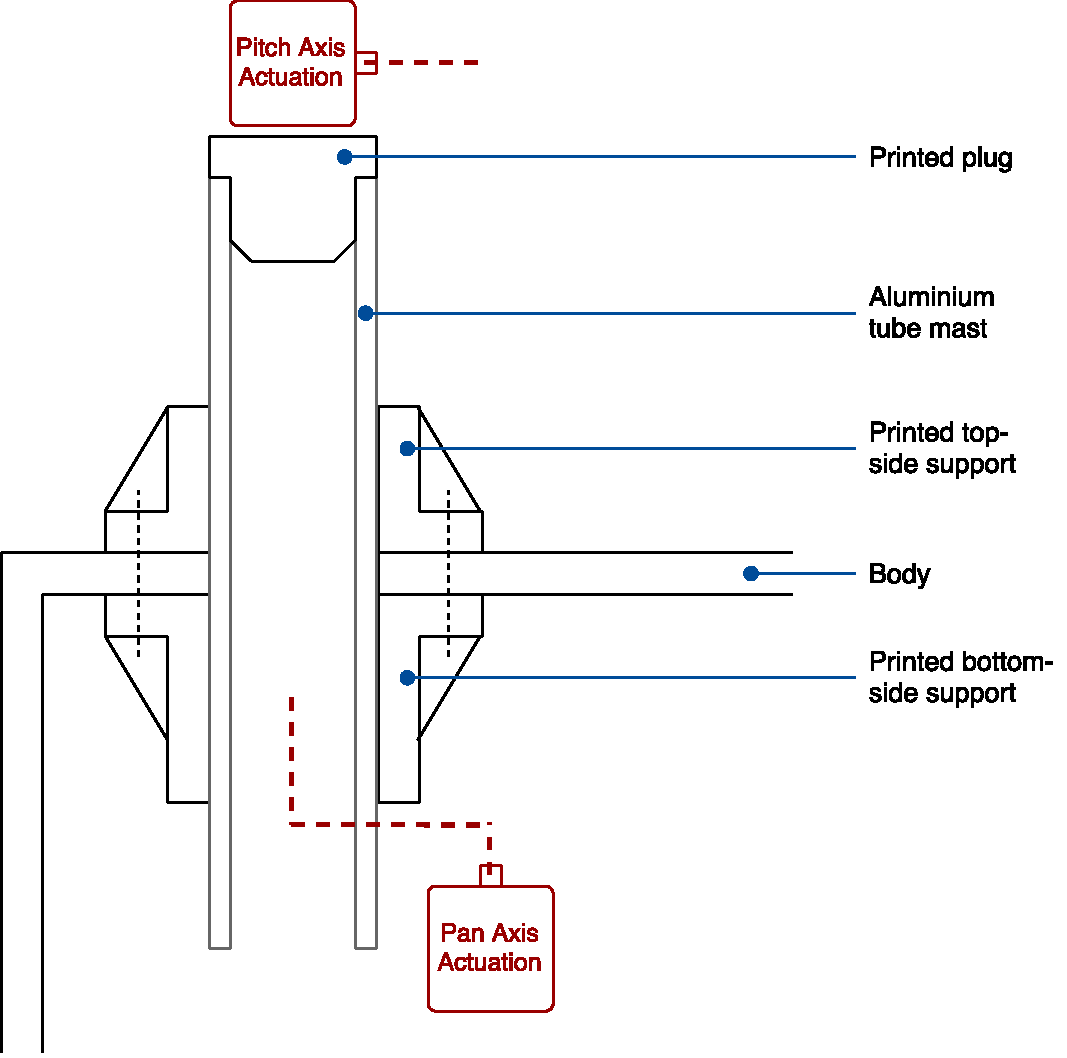
\includegraphics[width=0.7\linewidth]{figures/concepts-aluMast}
          \caption[Conceptual diagram of a section view of the body and aluminium mast assembly.]{Conceptual diagram of a section view of the body and aluminium mast assembly.}
          \label{fig:concepts-aluMast}
        \end{figure}
        
        \item \textbf{Full 3D Printed Assembly:} As opposed to making use of aluminium tubing, this concept employs 3D printing for the full assembly which would be mounted to the top of the rover body with no portion of it extending below the deck. The camera-pan actuation would be the same as in the previous concept but the camera-pitch actuation mechanism would be brought above the level of the rover deck. Further, an actuation mechanism that combines both axes of motion could have been developed to reduce the spatial footprint that it might have incurred. The width of the base of the mast, at the mounting point, would be increased to provide structural support.
        
        \begin{figure}[H]
          \centering
          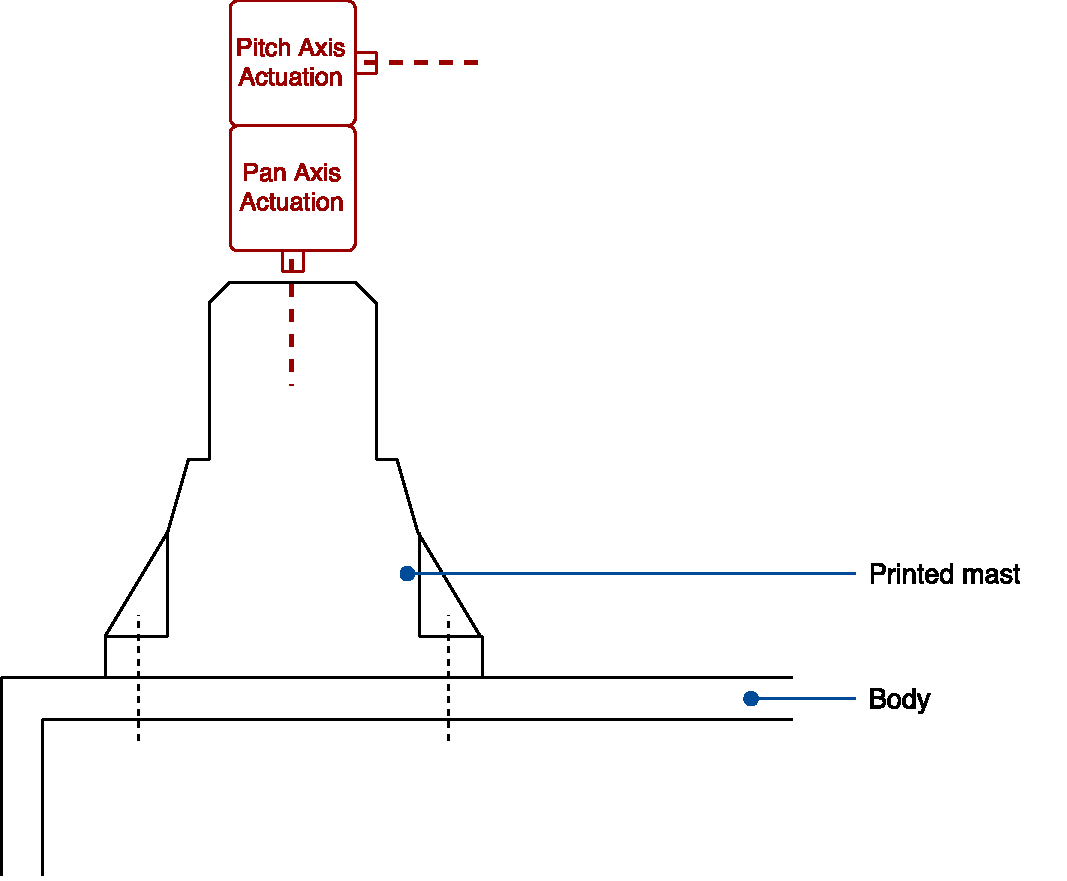
\includegraphics[width=0.7\linewidth]{figures/concepts-printedMast}
          \caption[Conceptual diagram of a section view of the body and printed mast assembly.]{Conceptual diagram of a section view of the body and printed mast assembly.}
          \label{fig:concepts-printedMast}
        \end{figure}
        
      \end{itemize}
      
      \subheading{Discussion}\\\\
        Positioning one of the two component actuation mechanisms inside the body had benefits for the spatial footprint above the rover deck, however, the implications of taking up more space inside the body were far greater given the intended use of that area. Having the entire tube mast rotate within the opening hole from below the deck might have increased the torque requirements on the actuation mechanism, dependant on the nature of the opening. The intended use of the opening was to provide structural support and any fit tolerance introduced to improve the torque requirements of the actuation would negatively impact the effectiveness of the hole feature in its support function. This could have been solved with a bearings, however, that would have incurred additional room for mounting.
      
      \subheading{Comparative Analysis}\\\\
      A comparative analysis of the two options for the construction of the neck and head assembly is shown in Table!\ref{tab:concept-compAnalysisMast}.
      
        \begin{table}[H]
        \centering
        \begin{tabular}{@{}L{0.3\textwidth}C{0.12\textwidth}C{0.2\textwidth}C{0.2\textwidth}@{}}
        \toprule
        Attribute & Weight & Aluminium Tube w/ 3D Printed Fittings & Full 3D Printed Assembly \\ \midrule
        Ease of Manufacture & 3 & 2 & 4 \\
        Duration of Manufacture & 4 & 4 & 3 \\
        Cost of Manufacture & 4 & 3 & 3 \\
        Cost of Material & 4 & 4 & 2 \\
        Weight & 4 & 3 & 4 \\
        Proportion & 3 & 4 & 3 \\
        Body External Footprint & 3 & 4 & 3 \\
        Body Internal Footprint & 5 & 1 & 5 \\
        Strength & 5 & 5 & 4 \\ \midrule
        \multicolumn{2}{r}{\textbf{Total}} & 3.200 & \textbf{3.514} \\ \bottomrule
        \end{tabular}
        \caption{Comparative analysis of the neck and head assembly concepts.}
        \label{tab:concept-compAnalysisMast}
        \end{table}
      
    \subsubsection{Actuation}
      All components requiring actuation mechanisms have been covered in the above concepts. Consisting of only rotational motion requirements, the mechanisms were split into two categories based on the desired order of output motion (translated from the desired order of input control signal), namely angular position and angular velocity. Position actuation was required for rotating the wheels about their $z$-axis pivot for turning or steering and to provide panning and pitching motion to the head subsystem with the camera. Both of the functions involved setting a desired angular position and having the mechanism hold that position during operation. On the other hand, driving the wheels of the rover was better thought as involving an output velocity. \textit{Curiosity} made use of high-ratio motors for all types of rotational actuation to ensure robustness of the design, higher torque outputs and to achieve precise control of each of the driven features which was acceptable in that high-speed performance was not a targeted requirement.
      
      \subheading{Concepts}
      \begin{itemize}
        \item \textbf{High Torque DC Motors:} Using high torque DC motors would have been the most accurate replication of the actuation as used on \textit{Curiosity}, as each of the mechanisms had high-ratio gearboxes attached to the brushless motors. The DC motors would have been controlled by means of PWM which would have resulted in an output angular velocity. For this reason, a control loop mechanism would have to be employed for positional motor control in the case of the subsystems that required it.
        \item \textbf{Analog RC Servos:} A candidate alternative to using high torque DC motors that was considered was servos, intended for radio-control vehicle use, into which a high-torque gearbox was already built. An example of this type of motor is shown in Figure~\ref{fig:concepts-servoMotorExample}. The motors operate using a pulse signal of which the width translated to a specific position as a percentage of the motor's rated angular range.
        
        \begin{figure}[H]
          \centering
          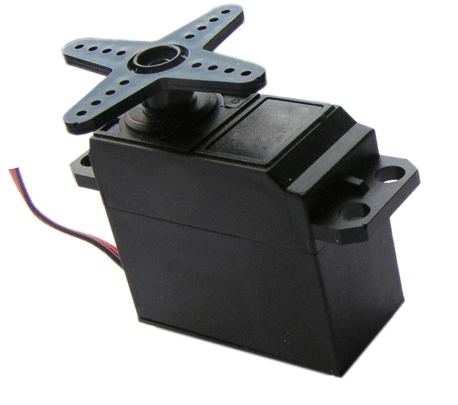
\includegraphics[width=0.3\linewidth]{figures/concepts-servoMotorExample}
          \caption[Image of an example of an RC servo motor.]{Image of an example of an RC servo motor \cite{fig:concepts-servoMotorExample_cite}.}
          \label{fig:concepts-servoMotorExample}
        \end{figure}

      \end{itemize}
      
      \subheading{Discussion}\\\\
        The two candidate actuation devices were in fact similar in that they both offered high torque output, however, the inclusion of a built-in analog position control system differentiated the servos from the DC motors. If the DC motors were to be used, the central system would had to provide an external control system to implement position control for the head and mast subsystem as well as the pivoting of the wheels. Further, this would have required output state capture by means of an encoder or an analog-to-digital converter adding complexity to the system. The fact that the servos had this control functionality built in meant this solution would have greatly reduced the incurred complexity of the actuation of the rover as a whole, as all that would have been required is for the system to provide a power rail and PWM signals.
        
        The choice of actuation mechanisms was highly dependant on the chosen combination of subsystem concepts, specifically that of the power supply, the central control system and those that needed actuation themselves. No weighted comparison was performed for the above concepts as the choice was heavily affected by these subsystems.
    
    \subsubsection{Central Control System}
    \label{subsubsec:central-control-system}
      The central control system was a critical component not only to the rover, but to the conceptual design process as it was an enabler/disabler of many of the candidate solutions. Discussed here are the electronic hardware comparisons made with respect to the central control system. The software design process took on a secondary priority approach and as such, the hardware choices were driving of the design (not without consideration of implications in the software system). As will be mentioned in full in the detailed design section, it was intended to follow a COTS design approach as far as possible given the time-frame of the project as well as the notion of keeping the design open to others who might be familiar with the hardware components chosen with respect to the aim of open sourcing. As far as education and outreach is concerned, familiar hardware is well suited to helping users and those involved in the project learn the principles of rover design.
      
      Conceptual candidate systems included popular, small, single-board computers, sized appropriately with the intention of fitting the system in the body of the model. Note that the lower-level device class suited to deeper embedded software applications was considered and would have proved suitable if it were not for the video streaming requirements. It was anticipated that the video feed would require on-rover encoding and compression and thus imposing the need for a better performing device capable of running a high-level operating system. The requirements for this system, which included wireless communication and embedded interfaces, were kept in mind when performing the comparative analysis. Notable specifications in accordance with the requirements are shown for each of the boards.
      
      \subheading{Concepts}
      \begin{itemize}
        \item \textbf{Raspberry Pi Model B:}
          The Raspberry Pi is a credit-card sized single-board computer which was developed with the intention of aiding computer-science education. It made use of a well-performing CPU as well as an on-chip GPU making it suitable for low-end, media-based computational applications. Raspberry Pi computers have a very large online community from which vast resources were available.
          
          Notable specifications (for the 3rd generation model):
          \begin{itemize}
            \item \textbf{CPU:} 1.2 GHz 64-bit ARM Cortex A53 (Broadcom BCM 2837 SoC)
            \item \textbf{Memory:} 1 GB
            \item \textbf{Storage:} None, microSD Card Slot
            \item \textbf{GPIOs:} 40 pins, 
            \item \textbf{Network Connectivity:} Bluetooth 4.1 and Bluetooth Low Energy, 100 Mb Ethernet, 2.4 GHz wireless
            \item \textbf{Other External Interfaces:} 4$\times$ USB 2.0, Camera Serial Interface (CSI)
          \end{itemize}
        \item \textbf{Orange Pi:}
          The Orange Pi, an open source variant to the Raspberry Pi, was considered as it offered much the same capabilities as the Rasberry Pi. It was able to run many open source operating systems such as Debian and Ubuntu.
          
          Notable specifications (for the Plus model):
          \begin{itemize}
            \item \textbf{CPU:} 1 GHz 64-bit ARM Cortex A7 (AllWinner H3 SoC)
            \item \textbf{Memory:} 1 GB
            \item \textbf{Storage:} None, microSD Card Slot, SATA 2.0 Connector
            \item \textbf{GPIOs:} 40 pin header, 
            \item \textbf{Network Connectivity:} 1 Gb Ethernet, 2.4 GHz wireless
            \item \textbf{Other External Interfaces:} 4$\times$ USB 2.0, Camera Serial Interface (CSI)
          \end{itemize}
          
        \item \textbf{Beaglebone Green Wireless:}
          The Beaglebone Green is another small board as part of the Beaglebone device family, a range of single-board computers that have been developed to bridge the gap between embedded electronics and computers. The green version is better suited for embedded applications compared to that of the black version and was the only Beaglebone device that had wireless connection capabilities.
          
          Notable specifications \cite{mouserbeaglebone_2016}:
          \begin{itemize}
            \item \textbf{CPU:} 1 GHz 32-bit ARM Cortex A8 (TI Sitara AM3358)
            \item \textbf{Memory:} 512 MB
            \item \textbf{Storage:} 4 GB eMMC
            \item \textbf{GPIOs:} 65 pins, 
            \item \textbf{Network Connectivity:} Bluetooth 4.1, Bluetooth Low Energy, 2.4 GHz wireless
            \item \textbf{Other External Interfaces:} 4$\times$ USB 2.0
          \end{itemize}
          
        \item \textbf{Intel Edison:}
          The Intel Edison is less of a single-board computer and more of a complete system on chip mounted to a small board intended for use in the Internet-of-Things industry as well as for mobile and wearable products. The tiny module can further be mounted to a breakout board which provides USB interfaces and a GPIO through-hole grid.

          Notable specifications \cite{intelEdison_2016}:
          \begin{itemize}
            \item \textbf{CPU:} 400 Mhz Intel Quark x86 (Intel Atom)
            \item \textbf{Memory:} 1 GB
            \item \textbf{Storage:} 4 GB eMMC
            \item \textbf{GPIOs:} 28 pins, 
            \item \textbf{Network Connectivity:} Bluetooth 4, 2.4 GHz wireless
            \item \textbf{Other External Interfaces:} 1$\times$ USB 2.0, 1$\times$ USB Serial (UART), as provided by the breakout board
          \end{itemize}
 
        \item \textbf{Intel Edison w/ Arduino Breakout Expansion:}
          The Intel Edison had available a second breakout board which was developed to make the SoC compatible with the large variety of Arduino-compatible modules and add-ons.

        \item \textbf{Intel Galileo Gen 2:}
          The Intel Galileo is a development board that better aligns with the single-board computer principle, compared to the Edison. The processor and board are fixed and allows for connection of Arduino-compatible hardware as well as supports a range of other interfaces.
          
          Notable specifications \cite{intelGalileo_2016}:
          \begin{itemize}
            \item \textbf{CPU:} 400 Mhz Intel Quark x86 (Intel Pentium)
            \item \textbf{Memory:} 256 MB
            \item \textbf{Storage:} None, SD Card Slot
            \item \textbf{Network Connectivity:} 1 Gb Ethernet Port
            \item \textbf{Other External Interfaces:} 3$times$ USB 2.0, 1$\times$ USB Serial (UART)
          \end{itemize}
      \end{itemize}
      
      \subheading{Discussion:}\\\\
        After careful research into each of the above candidate products, it was decided that all of the boards were suitable for the central computing system of the rover. All of the devices were capable of running high-level operating systems as well as had some means of connecting to a video capture device as well as providing hardware interfaces that might have been required. However, caution was taken to choose a device that would not be over-powered for the application nor provide breakouts and interfaces that would have been left unused. At this point in the design process, it was difficult to determine the exact computational requirements and so the design choice was made based on anticipative measures. It must be noted that the choice was also strongly influenced by availability and cost of the devices.
        
        \begin{table}[H]
        \centering
        \begin{tabular}{@{}L{0.15\textwidth}C{0.1\textwidth}C{0.1\textwidth}C{0.1\textwidth}C{0.1\textwidth}C{0.1\textwidth}C{0.1\textwidth}C{0.1\textwidth}@{}}
        \toprule
        Attribute & Weight & R-Pi 3 & Orange Pi & Beaglebone Green Wireless & Intel Edison & Intel Edison w/ Arduino Breakout & Intel Galileo Gen 2 \\ \midrule
        Cost & 5 & 4 & 4 & 3 & 2 & 2 & 1 \\
        \rule{0pt}{2em}Weight & 3 & 4 & 3 & 4 & 5 & 5 & 4 \\
        \rule{0pt}{2em}Availability & 5 & 3 & 1 & 2 & 5 & 4 & 5 \\
        \rule{0pt}{2em}Size & 4 & 4 & 3 & 4 & 5 & 4 & 3 \\
        \rule{0pt}{2em}Wireless Support & 5 & 5 & 5 & 5 & 5 & 5 & 0 \\
        \rule{0pt}{2em}Provision for Video Capture & 5 & 5 & 5 & 4 & 1 & 3 & 3 \\
        \rule{0pt}{2em}Suitability of Processing Power & 3 & 3 & 3 & 3 & 5 & 5 & 3 \\
        \rule{0pt}{2em}Add-on Compatibility & 4 & 3 & 3 & 2 & 1 & 5 & 5 \\
        \rule{0pt}{2em}Power Consumption & 3 & 1 & 1 & 3 & 5 & 4 & 2 \\ \midrule
        \multicolumn{2}{r}{\textbf{Total}} & 3.703 & 3.243 & 3.351 & 3.622 & \textbf{4.000} & 2.811 \\ \bottomrule
        \end{tabular}
        \caption{Comparative analysis of the central control system concepts.}
        \label{tab:concept-compAnalysisRce}
        \end{table}

      
    \subsubsection{Camera}
      An important item in the list of requirements and specifications was the capture of a video stream to broadcast to the connected clients. The camera was required to be above VGA resolution ($640\times480$ pixels) and have a means of connecting to the chosen central computing system. The available camera modules were categorised by connector type, listed below.
      
      \subheading{Concepts}
      \begin{itemize}
        \item \textbf{CSI Compatible Webcam:} Many of the central computing system candidates provided support for a Camera Serial Interface (CSI) connected camera for video capture. CSI is a camera interface standard maintained by the Mobile Industry Processor Interface Alliance (MIPI Alliance) that is at its 3rd stage of revision at the time of writing. An example of a CSI camera was the R-Pi Cam, produced specifically for use with a Raspberry Pi.
        \item \textbf{USB Compatible Webcam:} The majority of external webcams were USB connected, allowing them to be easily connected to a laptop or computer. The USB webcams that were investigated as being candidate devices varied in their class of drivers which was a potential issue for compatibility with the central control system, specifically the operating system that would be used. The chosen device, if of type USB, would have had to have been a USB Video Class (UVC) compliant device due to the fact that UVC devices are driverless and thus are compatible with a far greater range of host computers and operating systems.
        \item \textbf{I$^2$C Webcam:} Since the central control system would be capable of allowing serial connections, cameras that were I$^2$C connected were considered.
      \end{itemize}
      
      \subheading{Discussion}\\\\
        The performance benefit of candidate cameras was not possible to determine based on their interface type, but rather the manufacturer and the designed specifications. It was decided that the camera be chosen based on compatibility with the central control system and local availability of such a device.
      
    \subsubsection{Proximity}
      As per \ref{li:probDef-spec-sensors-immediateObstacleData}, the RCE required sensory data to implement elementary obstacle detection representative of the advanced navigational systems on \textit{Curiosity}. The sensors were to interface with the RCE board and have reasonable dimensions such that they could be positioned on the body and head module of the rover. A few candidates are listed by principle of operation below.
      
      \subheading{Concepts}
      \begin{itemize}
        \item \textbf{Ultrasonic:} Sensors of the ultrasonic or sonar type emit directional bursts of ultrasonic sound and measure the time taken for the echoes of said bursts to reach the sensor interface as an indication of the distance between the interface and the obstacle reflecting the sound-waves. A popular ultrasonic sensor module is the HC-SR04 (shown in Figure~\ref{fig:concepts-hcsr04}) which comprises of the transmitter and receiver components as well as circuitry which converts the measured time into a usable signal.
        
        \begin{figure}[h!]
          \centering
          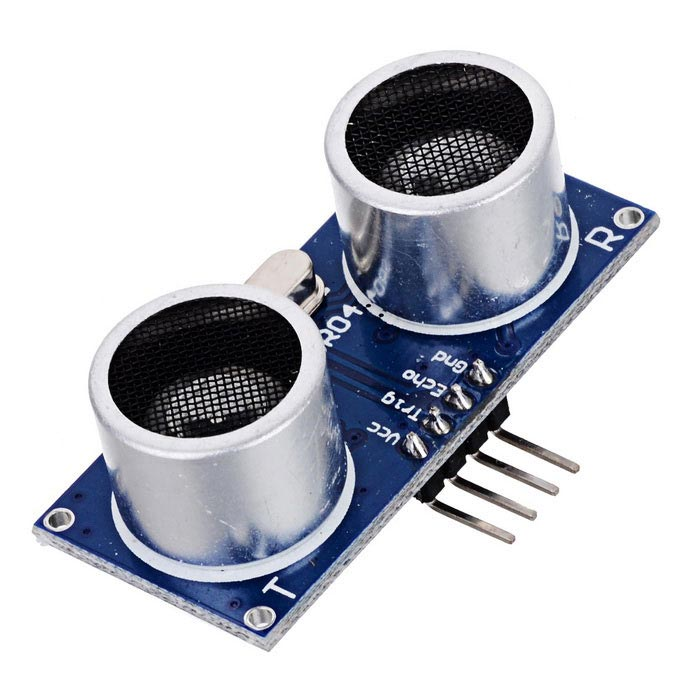
\includegraphics[width=0.4\linewidth]{figures/concepts-hcsr04}
          \caption[Image of the interface end of the HC-SR04 ultrasonic sensor module.]{Image of the interface end of the HC-SR04 ultrasonic sensor module \cite{fig:concepts-hcsr04_cite}.}
          \label{fig:concepts-hcsr04}
        \end{figure}
 
        \item \textbf{Infra-red:} Infra-red ranging sensors can work in two different ways, with different levels of accuracy as a result. The least accurate form is that which emit an infra-red beam and measure the intensity of the reflection of the beam. The second type involves the same emission of infra-red light. However, the measurement is not the intensity of the reflection but rather the angle at which it enters the sensor interface. This type of measurement is suited for accurate range finding and an example of such a sensor is the Sharp GP2Y0A21 shown in Figure~\ref{fig:concepts-sharpIR}.
        
        \begin{figure}[h!]
          \centering
          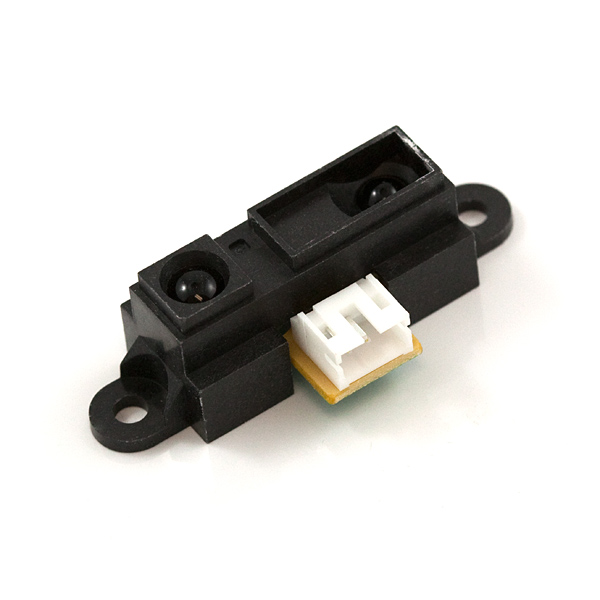
\includegraphics[width=0.4\linewidth]{figures/concepts-sharpIR}
          \caption[Image of the Sharp GP2Y0A21 infra-red ranging sensor.]{Image of the Sharp GP2Y0A21 infra-red ranging sensor \cite{fig:concepts-sharpIR_cite}.}
          \label{fig:concepts-sharpIR}
        \end{figure}
        
        
        \item \textbf{LiDAR:} LiDAR (Light Detection and Ranging) devices operate in a similar fashion to ultrasonic sensors, however, they make use of light bursts as opposed to sound bursts to make ranging measurements. As such, these devices can be directional and more accurate then the other two types of sensors. An example of a LiDAR sensor is the LIDAR-Lite 3 as shown in Figure~\ref{fig:concepts-lidarlite3}.
        
        \begin{figure}[h!]
          \centering
          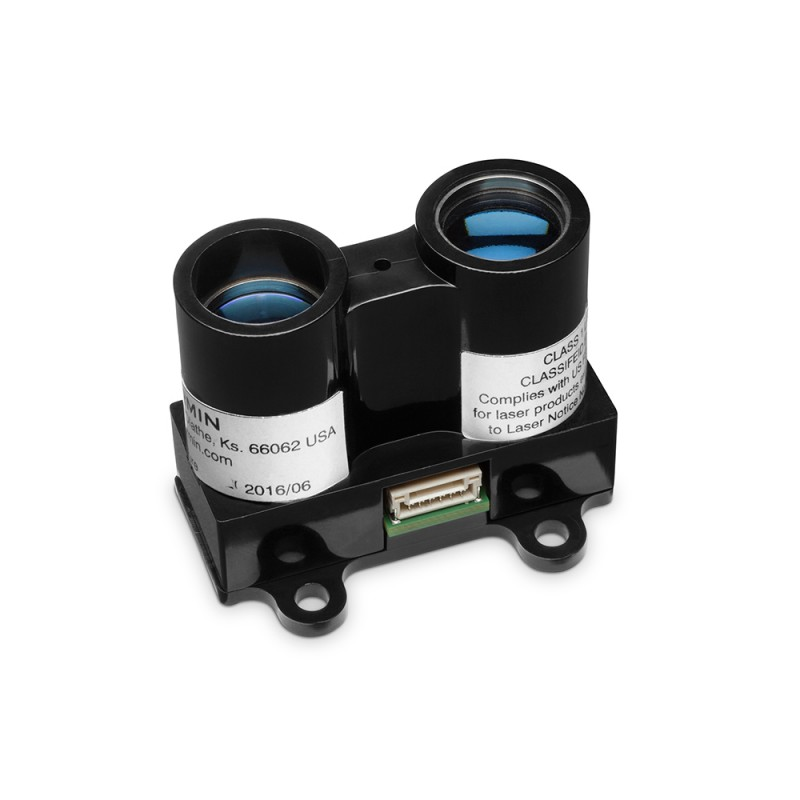
\includegraphics[width=0.4\linewidth]{figures/concepts-lidarLite3}
          \caption[Image of the LIDAR-Lite 3 optical ranging sensor.]{Image of the LIDAR-Lite 3 optical ranging sensor \cite{fig:concepts-lidarlite3_cite}.}
          \label{fig:concepts-lidarlite3}
        \end{figure}
        
      \end{itemize}
      
      \subheading{Comparative Analysis}\\\\
      A comparative analysis of the three options for the choice of a means of proximity sensing is shown in Table~\ref{tab:concept-compAnalysisProximity}.
      
      \begin{table}[h!]
      \centering
      \begin{tabular}{@{}L{0.2\textwidth}C{0.15\textwidth}C{0.15\textwidth}C{0.15\textwidth}C{0.15\textwidth}@{}}
      \toprule
      Attribute                 & Weight & Ultrasonic     & Infra-red & LiDAR \\ \midrule
      Cost                      & 5      & 5              & 4         & 2     \\
      Weight                    & 3      & 4              & 5         & 4     \\
      Availability              & 5      & 5              & 3         & 1     \\
      Size                      & 4      & 4              & 5         & 4     \\
      Accuracy                  & 2      & 4              & 2         & 5     \\
      Environmental Suitability & 4      & 5              & 1         & 5     \\ \midrule
      \multicolumn{2}{r}{\textbf{Total}} & \textbf{4.609} & 3.391     & 3.174 \\ \bottomrule
      \end{tabular}
      \caption{Comparative analysis of the proximity sensor types.}
      \label{tab:concept-compAnalysisProximity}
      \end{table}
      
      \subheading{Discussion}\\\\
        Although an appealing feature, accurate distance measurements were not required for the basic obstacle avoidance described in the technical specifications and so the use of the LiDAR sensor would have amounted to a costly over-design. Due to the fact that the ultrasonic sensor type combined a balance between availability and accuracy as well as being suitable for multiple environments, unlike the infra-red type, made it a preferred choice for the distance measurement system on the rover.
      
  
  \subsection{Final Design Choice}
    At this point, the ideas and concepts in Section~\ref{subsec:rover-concept-proposals} had been explored in detail and final choices for each of the subcomponents had been made. This section indicates the outcomes of these choices as well as gives a brief overview of the final concept to be developed. The subcomponent concepts in Section~\ref{subsec:rover-concept-proposals}, shown visually in Figure~\ref{fig:concepts-finalconceptrender}, that included weighted comparisons were finalised primarily by the outcome of those comparisons (i.e. the concept that achieved the highest score, denoted in the Tables~\ref{tab:concept-compAnalysisBody} through~\ref{tab:concept-compAnalysisRce} by bold numbers) and the few that did not follow the same structure of analysis were chosen by compatibility with relevant subcomponents.
    
    \begin{figure}[H]
      \centering
      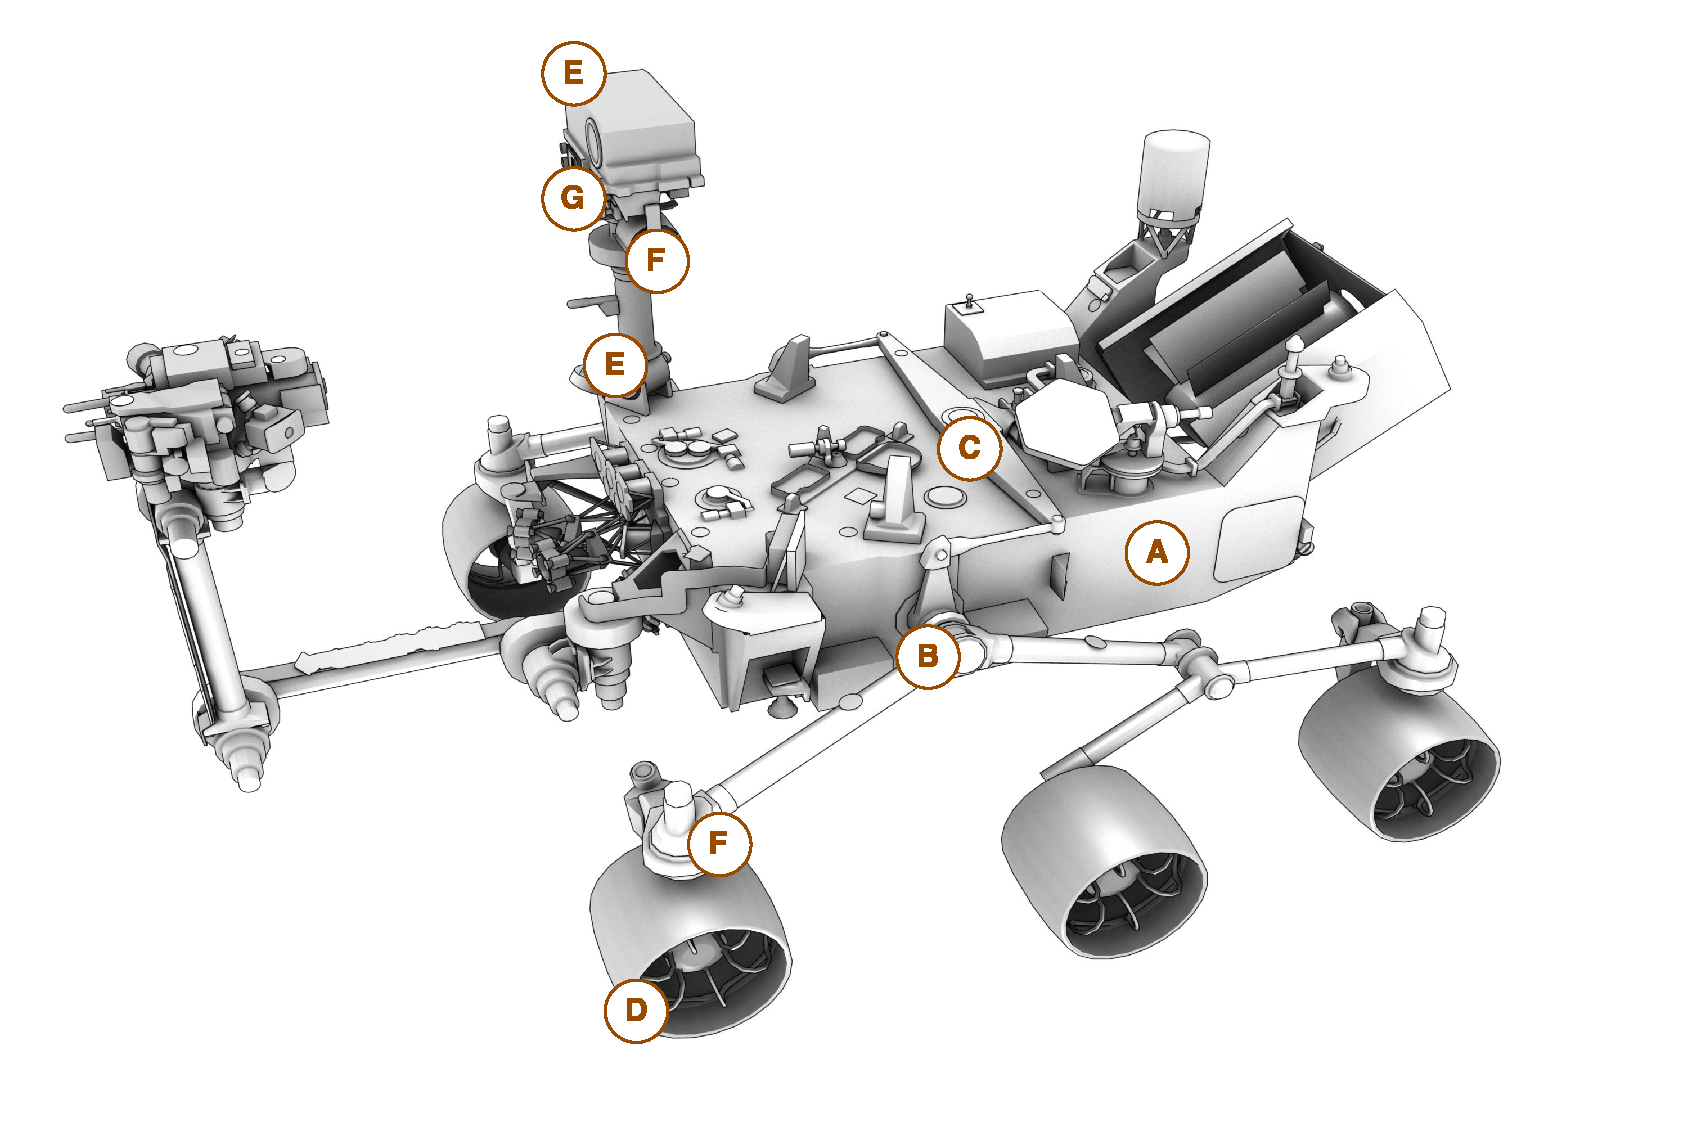
\includegraphics[width=1\linewidth]{figures/concepts-finalConceptRender}
      \caption[Adapted render of a model of the rover indicating the subsystems considered in the conceptual development.]{Adapted render of a model of the rover indicating the subsystems considered in the conceptual development \cite{nasa3D}.}
      \label{fig:concepts-finalconceptrender}
    \end{figure}
    
    \begin{enumerate}[label=\Alph*.]
      \item It was decided that the body be made from acrylic sheet panels glued together to form the box structure. The panel design, cutting and assembly was considered easier compared to the manufacturing carbon fibre on 3D printing, as well as being strong enough to provide the central structural support.
      \item The suspension system was to be constructed from 3D printed joints and aluminium tubing respecting the minimisation of weight of the assembly and the concept's compatibility with fittings to be made for mounting the wheels. The fact that the joints were to be 3D printed meant that it would become easy to model and print the required angles of the \textit{Curiosity} suspension design without the manufacturing limitations imposed by other methods and materials. The joints allowed for the design to maintain an accurate representation of that on \textit{Curiosity} without sacrificing function. This approach also meant that close fit parts such as bearings could be easily incorporated into the design without imposing constraints on the choice of those types of parts.
      \item A full 3D printed bar with printed hinges was to be used for the differential system due to the acrylic sheet and steel cord not being suitable for the required function. As mentioned in the discussion of the design concept, the 3D printed differential bar meant that a bearing could be correctly mounted for the motion required. The hinge on the differential bar side would be connected to the suspension side hinge by a threaded bar. As will be discussed, the connecting threaded bar could be used to adjust the distance between the hinges thus providing the ability to balance the rover finely during assembly.
      \item The wheels were to be 3D printed which would allow for superior aesthetic accuracy and custom fit design for bearings and actuation. The 3D printed wheels would also be lighter than bought wheels. Because of these advantages, 3D printing of the wheels was deemed worth the incurred manufacturing time and cost.
      \item The head and neck (mast) was to be fully 3D printed to make it more suitable for mounting on top of the rover deck without any portion of it extending into the body of the rover, taking up space required for the electronics. 3D printing meant the ability to accommodate for the chosen means of actuation. The head would be designed to consist of two parts so that access to the internal components of the head was possible. This sub-assembly was then to be mounted to parts connected to the actuation and further parts for mounting on the rover deck.
      \item Choice of actuation settled upon the use of RC servos. The servos were to be of a suitable size, preferably ``sub-micro''\footnote{A ``sub-micro'' servo motor is one of a range of standard sized servos for robotics and radio-controlled vehicle applications.}, and compatible in interface with the central control system. The servos chosen were highly geared to provide the required torque for actuation of the head and wheels. The servos would have standard mounting holes making incorporation into the design an easier process.
      \item The camera was to be a USB (UVC-compatible) webcam chosen based on availability. The camera would be suitable for use with the chosen central control system and significantly lower in cost compared to the other concept options. It was decided that a webcam be physically altered to be suitable for incorporation into the design of the head.
    \end{enumerate}
    
    Not shown in Figure~\ref{fig:concepts-finalconceptrender} is the central control system, which was to be mounted on the inside of the body structure. The Intel Edison with the Arduino breakout expansion was chosen due to availability of the product as well as its compatibility with add-on hardware, the advantage of which was in the increased development process as a result. The Intel Edison was regarded as being better suited to the performance and computational requirements over the other boards and provided the necessary hardware interfaces for the primary functions and associated hardware for the system throughout.
    
    As discussed in the functional analysis, \textit{Curiosity's} robotic arm subsystem was not included in the model due to time and cost constraints on the project. However, the design allows the addition of this subsystem in the future.

    